\documentclass[aps,pre,preprint,notitlepage,nofootinbib,superscriptaddress]{revtex4-2}

\usepackage[T1]{fontenc}
\usepackage{lmodern}
\usepackage{microtype}
\usepackage{amsmath,amssymb,mathtools,bm,mathrsfs,amsthm}
\usepackage{booktabs,array}
\usepackage{siunitx}
\usepackage{tikz}
\usetikzlibrary{arrows.meta,calc,decorations.markings,decorations.pathmorphing,positioning,shapes.geometric,fit,backgrounds}
\usepackage{hyperref}
\usepackage[nameinlink,noabbrev]{cleveref}
\usepackage{xcolor}
\usepackage{enumitem}

\hypersetup{
  colorlinks=true,
  linkcolor=blue!55!black,
  citecolor=blue!55!black,
  urlcolor=blue!55!black,
  pdftitle={Transverse Projection and Finite-Core Response of Tight Knotted Vortex Tubes},
  pdfauthor={Omar Iskandarani},
  pdfsubject={Geometric identities and finite-core response of tight knotted vortex tubes},
  pdfkeywords={vortex dynamics, ropelength, ideal knots, helicity, Biot-Savart energy, gauge coupling}
}

\sisetup{separate-uncertainty=true, per-mode=symbol}
\newcommand{\dd}{\mathrm d}
\newcommand{\RR}{\mathbb R}
\newcommand{\Rop}{\operatorname{Rop}}
\newcommand{\FP}{\operatorname{FP}}
\newcommand{\Tr}{\operatorname{Tr}}
\newcommand{\e}{\mathrm e}
\newcommand{\ii}{\mathrm i}
\newcommand{\calH}{\mathcal H}
\newcommand{\calL}{\mathcal L}
\newcommand{\calR}{\mathcal R}
\newcommand{\calI}{\mathcal I}
\newcommand{\calC}{\mathcal C}
\newcommand{\calE}{\mathcal E}
\newcommand{\Rmicro}{\mathscr R_{\mathrm{micro}}}
\newcommand{\Rgeom}{\mathscr R_{0}}
\newcommand{\Reff}{\mathscr R_{\mathrm{eff}}}
\newcommand{\unitvec}[1]{\widehat{\bm #1}}

\newtheorem{proposition}{Proposition}
\newtheorem{corollary}{Corollary}
\newtheorem{hypothesis}{Matching hypothesis}
\newtheorem{remark}{Remark}

\begin{document}

\title{\texorpdfstring{Transverse Projection and Finite-Core Response of Tight Knotted Vortex Tubes\\\large Geometric identities, helicity constraints, and an open gauge-stiffness matching problem}{Transverse Projection and Finite-Core Response of Tight Knotted Vortex Tubes: Geometric identities, helicity constraints, and an open gauge-stiffness matching problem}}

\author{Omar Iskandarani}
\email{info@omariskandarani.com}
\thanks{ORCID: 0009-0006-1686-3961}
\affiliation{Independent Researcher, Groningen, The Netherlands}
\date{2 August 2026}

\begin{abstract}
A closed vortex tube combines three structures that are often conflated: the geometry of its centerline, the internal structure of its finite core, and the normalization of any long-distance field to which it may couple.  This paper separates these layers.  First, the incompressible Fourier-space projector is averaged over all propagation directions.  For every unit tangent $\bm t$,
\[
\int_{S^2} t_i(\delta_{ij}-\widehat{k}_i\widehat{k}_j)t_j\,\dd\Omega=\frac{8\pi}{3}.
\]
Consequently, a diameter-normalized tube centerline of length $L$ defines the exact geometric response $\Rgeom=(8\pi/3)(L/D)$.  The same factor follows from a normalized constant-radius tube volume, but neither construction generates a curvature correction: the bare local projector is orientation independent, and the curvature term in the tube Jacobian vanishes after angular integration.  A nonzero correction must therefore arise from finite-core dynamics, material-frame twist, or nonlocal self-interaction.

Starting from the kinetic energy of an incompressible Euler flow, the standard vorticity and filament representations are derived, leading to the regularized Biot--Savart energy of a closed vortex tube.  A low-energy finite-core expansion is then organized in curvature, material twist, and contact operators.  For a single framed thin tube, helicity constrains the topological sector through $\calH/\Gamma^2=SL=Wr+Tw$.  Cauchy--Schwarz yields the parity-even bound
\[
\calI_{\Omega^2}\ge \frac{4\pi^2}{\calL_D}(SL-Wr)^2,
\]
with equality only for uniform material twist.  Thus helicity constrains a quadratic twist energy; it does not supply a linear correction to a parity-even gauge kinetic term.

Numerical trefoil data are used only as a convention and provenance test.  The high-resolution radius-normalized ropelength $32.742934477$ is equivalent to the diameter-normalized value $16.3714672385$; a Fourier database value $16.371637$ defines a distinct numerical branch.  Their proximity is strong evidence for scalar ropelength convergence but not for convergence of finite-core response.  Finally, an electromagnetic interpretation is formulated as an explicitly open matching problem: a dimensionless response may be identified with an inverse gauge coupling only after the gauge field and source current have been independently normalized and a genuine $U(1)$ sector with two physical transverse modes has been established.  A calibration and holdout protocol is given that forbids reuse of the target coupling or equivalent calibration data.
\end{abstract}

\keywords{vortex dynamics, ropelength, ideal knots, transverse projector, helicity, writhe, twist, Biot--Savart energy, effective field theory, gauge coupling}

\maketitle

\section{Introduction}

Knotted vortex tubes are simultaneously geometric objects, solutions or approximate solutions of fluid equations, and potential carriers of topological invariants.  These roles should be distinguished.  Ropelength is a scale-invariant property of an embedded centerline with nonzero thickness.  Helicity is a conserved integral of a solenoidal field under ideal evolution.  Kinetic energy depends on the entire velocity or vorticity distribution, including the core profile and nonlocal induction.  A gauge coupling, in contrast, is defined only after both the gauge kinetic term and the normalization of charged sources have been fixed.

The purpose of this paper is to isolate a precise chain of statements that can be assessed independently:
\begin{enumerate}[label=(\roman*)]
  \item an exact angular identity associated with the incompressible transverse projector;
  \item its conversion into a length-normalized geometric response;
  \item two no-go results showing why the same local constructions cannot provide a geometry-sensitive correction;
  \item the orthodox Euler--Biot--Savart energy and its finite-core regularization;
  \item the role of helicity, writhe, and material twist in a parity-even response;
  \item the additional normalization conditions required before any response coefficient can be interpreted as an electromagnetic coupling.
\end{enumerate}

No microscopic derivation of the electromagnetic fine-structure constant is claimed.  The comparison with its inverse value is retained only as a numerical target that motivates an independent calibration experiment.  In particular, the target value, the elementary charge, and any parameter previously calibrated through the target coupling are excluded from the finite-core matching stage.

The geometric part of the analysis is grounded in established ropelength theory.  Ropelength minimizers exist in each tame knot type and are $C^{1,1}$, but they need not be $C^2$ or unique \cite{CantarellaKusnerSullivan2002}.  Constrained-gradient computations make the active strut and kink constraints explicit \cite{AshtonCantarellaPiatekRawdon2011}.  High-resolution work on the trefoil shows that scalar length alone conceals nontrivial curvature, torsion, and contact structure \cite{PrzybylPieranski2014}.  These facts motivate the use of material frames and finite-core operators rather than unregularized Frenet torsion.

\section{Geometric preliminaries and conventions}
\label{sec:geometry}

Let $\gamma:S^1\to\RR^3$ be a closed embedded curve parameterized by arclength $s$, with unit tangent
\begin{equation}
  \bm t(s)=\frac{\dd\bm\gamma}{\dd s},\qquad |\bm t|=1.
\end{equation}
Let $a$ denote the radius of an embedded normal tube around $\gamma$, and let $D=2a$ be its diameter.  The standard radius-normalized ropelength is
\begin{equation}
  \Rop_a[\gamma]=\frac{L}{a},
\end{equation}
whereas the diameter-normalized length used below is
\begin{equation}
  \calL_D[\gamma]=\frac{L}{D}=\frac12\Rop_a[\gamma].
  \label{eq:diameter-normalized}
\end{equation}
The distinction is elementary but numerically decisive: multiplying a radius-normalized ropelength by a coefficient derived for $L/D$ introduces an erroneous factor of two.

\begin{figure}[t]
\centering
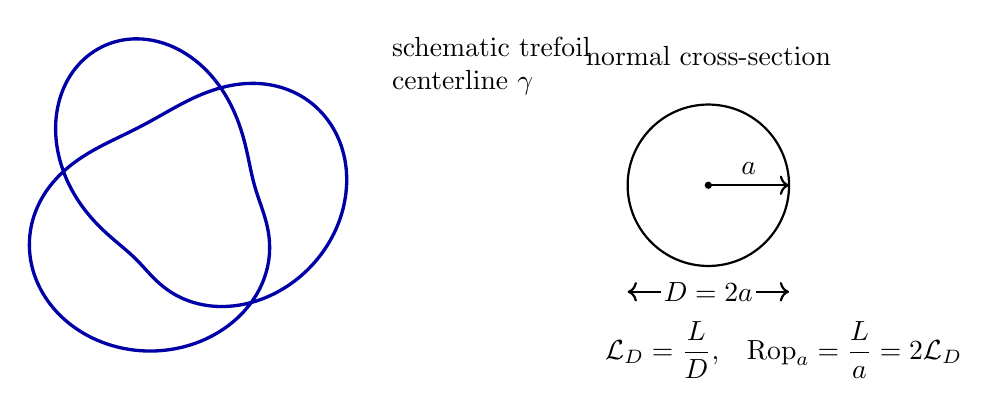
\begin{tikzpicture}[scale=0.82]
  \draw[very thick,blue!65!black,line cap=round,line join=round]
    plot[smooth] coordinates {(2.5840,0.0000) (2.5990,0.1886) (2.5938,0.3746) (2.5688,0.5556) (2.5244,0.7293) (2.4618,0.8935) (2.3820,1.0461) (2.2866,1.1856) (2.1773,1.3104) (2.0561,1.4195) (1.9248,1.5122) (1.7856,1.5881) (1.6405,1.6471) (1.4915,1.6896) (1.3405,1.7161) (1.1894,1.7275) (1.0397,1.7251) (0.8926,1.7101) (0.7495,1.6840) (0.6110,1.6486) (0.4779,1.6054) (0.3503,1.5562) (0.2282,1.5024) (0.1116,1.4458) (-0.0000,1.3875) (-0.1074,1.3288) (-0.2111,1.2706) (-0.3121,1.2137) (-0.4113,1.1584) (-0.5097,1.1049) (-0.6080,1.0531) (-0.7071,1.0026) (-0.8076,0.9529) (-0.9100,0.9032) (-1.0146,0.8524) (-1.1214,0.7995) (-1.2302,0.7433) (-1.3404,0.6826) (-1.4514,0.6161) (-1.5621,0.5429) (-1.6714,0.4618) (-1.7777,0.3720) (-1.8794,0.2730) (-1.9749,0.1644) (-2.0621,0.0459) (-2.1394,-0.0821) (-2.2048,-0.2192) (-2.2565,-0.3645) (-2.2929,-0.5170) (-2.3125,-0.6754) (-2.3141,-0.8379) (-2.2967,-1.0027) (-2.2596,-1.1679) (-2.2026,-1.3311) (-2.1255,-1.4903) (-2.0290,-1.6431) (-1.9136,-1.7873) (-1.7806,-1.9208) (-1.6314,-2.0415) (-1.4679,-2.1477) (-1.2920,-2.2378) (-1.1061,-2.3105) (-0.9126,-2.3649) (-0.7142,-2.4003) (-0.5134,-2.4165) (-0.3131,-2.4135) (-0.1157,-2.3917) (0.0761,-2.3519) (0.2602,-2.2953) (0.4343,-2.2230) (0.5966,-2.1369) (0.7457,-2.0385) (0.8801,-1.9300) (0.9992,-1.8132) (1.1023,-1.6903) (1.1894,-1.5634) (1.2606,-1.4343) (1.3164,-1.3049) (1.3576,-1.1768) (1.3853,-1.0516) (1.4008,-0.9304) (1.4055,-0.8141) (1.4011,-0.7033) (1.3890,-0.5984) (1.3709,-0.4995) (1.3485,-0.4062) (1.3231,-0.3181) (1.2962,-0.2344) (1.2687,-0.1542) (1.2418,-0.0765) (1.2160,-0.0000) (1.1918,0.0765) (1.1692,0.1542) (1.1482,0.2344) (1.1284,0.3181) (1.1091,0.4062) (1.0895,0.4995) (1.0686,0.5984) (1.0452,0.7033) (1.0182,0.8141) (0.9862,0.9304) (0.9479,1.0516) (0.9022,1.1768) (0.8480,1.3049) (0.7844,1.4343) (0.7106,1.5634) (0.6262,1.6903) (0.5309,1.8132) (0.4248,1.9300) (0.3083,2.0385) (0.1820,2.1369) (0.0470,2.2230) (-0.0956,2.2953) (-0.2442,2.3519) (-0.3972,2.3917) (-0.5525,2.4135) (-0.7082,2.4165) (-0.8621,2.4003) (-1.0122,2.3649) (-1.1561,2.3105) (-1.2920,2.2378) (-1.4178,2.1477) (-1.5319,2.0415) (-1.6327,1.9208) (-1.7189,1.7873) (-1.7896,1.6431) (-1.8441,1.4903) (-1.8822,1.3311) (-1.9038,1.1679) (-1.9093,1.0027) (-1.8995,0.8379) (-1.8751,0.6754) (-1.8375,0.5170) (-1.7882,0.3645) (-1.7286,0.2192) (-1.6606,0.0821) (-1.5860,-0.0459) (-1.5065,-0.1644) (-1.4240,-0.2730) (-1.3403,-0.3720) (-1.2567,-0.4618) (-1.1748,-0.5429) (-1.0956,-0.6161) (-1.0200,-0.6826) (-0.9487,-0.7433) (-0.8820,-0.7995) (-0.8199,-0.8524) (-0.7621,-0.9032) (-0.7081,-0.9529) (-0.6570,-1.0026) (-0.6080,-1.0531) (-0.5597,-1.1049) (-0.5109,-1.1584) (-0.4601,-1.2137) (-0.4059,-1.2706) (-0.3468,-1.3288) (-0.2815,-1.3875) (-0.2088,-1.4458) (-0.1276,-1.5024) (-0.0371,-1.5562) (0.0632,-1.6054) (0.1736,-1.6486) (0.2941,-1.6840) (0.4243,-1.7101) (0.5635,-1.7251) (0.7106,-1.7275) (0.8644,-1.7161) (1.0231,-1.6896) (1.1851,-1.6471) (1.3482,-1.5881) (1.5101,-1.5122) (1.6687,-1.4195) (1.8215,-1.3104) (1.9662,-1.1856) (2.1005,-1.0461) (2.2224,-0.8935) (2.3297,-0.7293) (2.4208,-0.5556) (2.4943,-0.3746) (2.5489,-0.1886) (2.5840,-0.0000)};
  \node[align=left,anchor=west] at (3.15,2.0)
    {schematic trefoil\\centerline $\gamma$};
  \begin{scope}[shift={(8.2,0.15)}]
    \draw[thick] (0,0) circle (1.25);
    \draw[<->,thick] (-1.25,-1.65)--(1.25,-1.65)
      node[midway,fill=white,inner sep=1pt] {$D=2a$};
    \draw[->,thick] (0,0)--(1.25,0)
      node[midway,above] {$a$};
    \fill (0,0) circle (1.6pt);
    \node[align=center] at (0,2.0) {normal cross-section};
    \node[align=left,anchor=west] at (-1.75,-2.55)
      {$\displaystyle \calL_D=\frac{L}{D}$,\quad
       $\displaystyle \Rop_a=\frac{L}{a}=2\calL_D$};
  \end{scope}
\end{tikzpicture}
\caption{A schematic trefoil centerline and the radius--diameter convention.  The plotted trefoil is not a numerical ropelength minimizer; it only illustrates the topology and normalization.}
\label{fig:trefoil-convention}
\end{figure}

For a $C^{1,1}$ minimizer, curvature exists almost everywhere and is essentially bounded.  By contrast, Frenet torsion may be ill-defined at inflection points or across nonsmooth transitions.  A physical twist variable should therefore be attached to a material or core director, not inferred from Frenet torsion alone.

\section{The isotropic transverse-projector identity}
\label{sec:projector}

In Fourier space, incompressibility requires
\begin{equation}
  k_i\widetilde u_i(\bm k)=0.
\end{equation}
The orthogonal projector onto the plane transverse to $\bm k$ is
\begin{equation}
  P_{ij}(\unitvec{k})=\delta_{ij}-\widehat k_i\widehat k_j.
  \label{eq:projector}
\end{equation}
For a fixed unit tangent $\bm t$,
\begin{equation}
  t_iP_{ij}t_j=1-(\bm t\cdot\unitvec{k})^2.
\end{equation}
Rotational invariance implies
\begin{equation}
  \int_{S^2}\widehat k_i\widehat k_j\,\dd\Omega
  =\frac{4\pi}{3}\delta_{ij}.
  \label{eq:isotropic-second-moment}
\end{equation}

\begin{proposition}[Isotropic transverse fraction]
For every unit vector $\bm t\in\RR^3$,
\begin{equation}
  \boxed{
  \int_{S^2}t_iP_{ij}(\unitvec{k})t_j\,\dd\Omega
  =\frac{8\pi}{3}.}
  \label{eq:8pi3}
\end{equation}
\end{proposition}

\begin{proof}
Using \cref{eq:isotropic-second-moment},
\begin{align}
  \int_{S^2}t_iP_{ij}t_j\,\dd\Omega
  &=4\pi-t_it_j\frac{4\pi}{3}\delta_{ij}\nonumber\\
  &=4\pi-\frac{4\pi}{3}|\bm t|^2
   =\frac{8\pi}{3}.
\end{align}
\end{proof}

The factor $3$ is therefore the denominator of the isotropic second moment in three spatial dimensions.  It is unrelated to the crossing number of the trefoil, its threefold visual symmetry, or any proposed periodic contact orbit.

\begin{figure}[t]
\centering
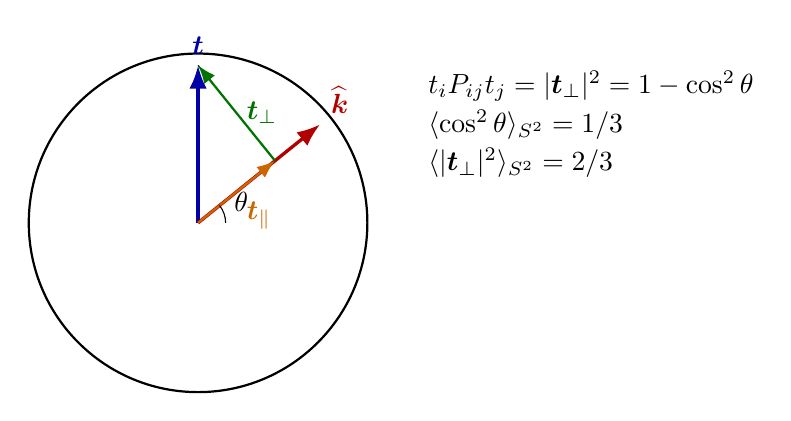
\begin{tikzpicture}[scale=1.0,>=Latex]
  \draw[thick] (0,0) circle (2.15);
  \draw[->,very thick,blue!65!black] (0,0)--(0,2.0) node[above] {$\bm t$};
  \draw[->,very thick,red!70!black] (0,0)--(1.55,1.25) node[above right] {$\unitvec{k}$};
  \coordinate (K) at (1.55,1.25);
  \draw[dashed] (0,2.0)--($(K)!(0,2.0)!(0,0)$);
  \coordinate (Q) at ($(K)!(0,2.0)!(0,0)$);
  \draw[->,thick,orange!80!black] (0,0)--(Q) node[midway,below right] {$\bm t_{\parallel}$};
  \draw[->,thick,green!45!black] (Q)--(0,2.0) node[midway,right] {$\bm t_{\perp}$};
  \draw (0.35,0) arc[start angle=0,end angle=39,radius=0.35];
  \node at (0.55,0.27) {$\theta$};
  \node[align=left,anchor=west] at (2.8,1.25)
    {$t_iP_{ij}t_j=|\bm t_\perp|^2=1-\cos^2\theta$\\[2pt]
     $\langle\cos^2\theta\rangle_{S^2}=1/3$\\[2pt]
     $\langle|\bm t_\perp|^2\rangle_{S^2}=2/3$};
\end{tikzpicture}
\caption{The transverse projector removes the component of $\bm t$ parallel to $\unitvec{k}$.  Isotropic averaging leaves the fraction $2/3$ of the squared unit tangent, and integration over the sphere gives $4\pi(2/3)=8\pi/3$.}
\label{fig:projector}
\end{figure}

\begin{corollary}[Length response]
Define
\begin{equation}
  \Rgeom[\gamma]
  :=\int_\gamma\frac{\dd s}{D}
     \int_{S^2}t_iP_{ij}t_j\,\dd\Omega.
\end{equation}
Then
\begin{equation}
  \boxed{
  \Rgeom[\gamma]=\frac{8\pi}{3}\calL_D
  =\frac{4\pi}{3}\Rop_a.}
  \label{eq:leading-response}
\end{equation}
\end{corollary}

\subsection{A local no-go result}

Equation \eqref{eq:8pi3} is independent of the local direction of $\bm t$.  It follows immediately that the bare local construction contains no information about curvature, torsion, writhe, contact, or core profile:
\begin{equation}
  \boxed{\Delta_{\mathrm{bare\ projector}}=0.}
  \label{eq:projector-no-go}
\end{equation}
Any geometry-sensitive correction must therefore modify the kernel being averaged or introduce additional finite-core and nonlocal variables.

\section{The constant-radius tube-volume identity}
\label{sec:tube-volume}

A second appearance of the same coefficient follows from the volume of an embedded tube.  For a sufficiently regular centerline, choose the Frenet-frame parameterization
\begin{equation}
  \bm x(s,r,\phi)=\bm\gamma(s)
  +r\cos\phi\,\bm n(s)+r\sin\phi\,\bm b(s).
\end{equation}
Before the normal tube self-overlaps, the volume element is
\begin{equation}
  \dd V=r\left(1-\kappa r\cos\phi\right)
  \dd r\,\dd\phi\,\dd s.
  \label{eq:tube-jacobian}
\end{equation}
Integrating over $0\le r\le a$ and $0\le\phi<2\pi$ gives
\begin{equation}
  V_{\mathrm{tube}}=\pi a^2L,
  \label{eq:tube-volume}
\end{equation}
because the term linear in curvature vanishes under the $\phi$ integral.  Hence
\begin{equation}
  \boxed{
  \frac{4}{3}\frac{V_{\mathrm{tube}}}{a^3}
  =\frac{4\pi L}{3a}
  =\frac{8\pi}{3}\calL_D.}
  \label{eq:tube-volume-identity}
\end{equation}

This identity is geometrically exact within its domain of validity, but it is not an electromagnetic derivation.  It also yields a second no-go statement:
\begin{equation}
  \boxed{\Delta_{\mathrm{constant\ tube\ volume}}=0.}
  \label{eq:tube-no-go}
\end{equation}
A nonzero correction from a tube construction requires at least one ingredient absent from \cref{eq:tube-jacobian}: a deformed or nonuniform cross-section, a spatially varying core profile, contact-mediated stress, overlap regularization, or another dynamical field.

\section{Euler energy in velocity and vorticity form}
\label{sec:euler-energy}

Consider an incompressible fluid of constant density $\rho$ in $\RR^3$ or in a domain with boundary conditions that eliminate the relevant surface terms.  The kinetic energy is
\begin{equation}
  E=\frac{\rho}{2}\int |\bm u(\bm x)|^2\,\dd^3x,
  \qquad \nabla\cdot\bm u=0.
  \label{eq:euler-velocity-energy}
\end{equation}
Introduce the vorticity $\bm\omega=\nabla\times\bm u$ and a vector potential
\begin{equation}
  \bm A(\bm x)=\frac{1}{4\pi}
  \int\frac{\bm\omega(\bm x')}{|\bm x-\bm x'|}\,\dd^3x',
  \qquad \bm u=\nabla\times\bm A.
\end{equation}
Integration by parts yields
\begin{equation}
  \int |\bm u|^2\,\dd^3x
  =\int \bm A\cdot\bm\omega\,\dd^3x,
\end{equation}
so that
\begin{equation}
  \boxed{
  E=\frac{\rho}{8\pi}
  \int\!\dd^3x\int\!\dd^3x'\,
  \frac{\bm\omega(\bm x)\cdot\bm\omega(\bm x')}
       {|\bm x-\bm x'|}.}
  \label{eq:vorticity-energy}
\end{equation}
This is the orthodox nonlocal energy functional for a solenoidal vorticity field \cite{Saffman1992,Moffatt1969}.

\subsection{Formal filament limit}

For a zero-radius filament of circulation $\Gamma$ supported on $\gamma$,
\begin{equation}
  \bm\omega(\bm x)=\Gamma\oint_\gamma
  \bm t(s)\,\delta^{(3)}\!\left(\bm x-\bm\gamma(s)\right)\dd s.
  \label{eq:filament-vorticity}
\end{equation}
Substitution into \cref{eq:vorticity-energy} gives
\begin{equation}
  \boxed{
  E_{\mathrm{BS}}[\gamma]
  =\frac{\rho\Gamma^2}{8\pi}
  \oint_\gamma\!\oint_\gamma
  \frac{\bm t(s)\cdot\bm t(s')}
       {|\bm\gamma(s)-\bm\gamma(s')|}
  \dd s\,\dd s'.}
  \label{eq:filament-energy}
\end{equation}
The diagonal $s=s'$ diverges.  Equation \eqref{eq:filament-energy} is therefore a formal filament expression, not a finite energy of a physical tube.  It must be replaced by a core-resolved vorticity distribution or by an explicitly stated regularization.

With $\bm X=\bm\gamma/D$ and $\sigma=s/D$, the natural energy scale is $\rho\Gamma^2D$ because
\begin{equation}
  [\rho\Gamma^2D]=\mathrm{kg\,m^2\,s^{-2}}.
\end{equation}
A generic dimensionless regularized functional can be written as
\begin{equation}
  \calE_f[\gamma]
  :=\frac{8\pi E_f}{\rho\Gamma^2D}
  =\FP\oint\!\dd\sigma\oint\!\dd\sigma'\,
  \bm t(\sigma)\cdot\bm t(\sigma')
  G_f\!\left(|\bm X(\sigma)-\bm X(\sigma')|\right),
  \label{eq:regularized-energy}
\end{equation}
where $f$ labels the core profile, $G_f$ is the corresponding regularized kernel, and $\FP$ denotes the declared subtraction or replacement of the local self-part.  Different profiles generally produce different finite constants and different higher-order response coefficients.

\section{Finite-core effective expansion}
\label{sec:effective-expansion}

At scales long compared with the core diameter, a regularized tube response may be organized as an effective expansion.  Let
\begin{equation}
  \widehat\kappa=D\kappa,
  \qquad
  \widehat\Omega=D\Omega_3,
\end{equation}
where $\Omega_3$ is the rotation rate of a material director about the tangent.  Define
\begin{equation}
  \calI_{\kappa^2}=\int_\gamma \widehat\kappa^2\,\frac{\dd s}{D},
  \qquad
  \calI_{\Omega^2}=\int_\gamma \widehat\Omega^2\,\frac{\dd s}{D}.
  \label{eq:operators}
\end{equation}
A minimal parity-even truncation is
\begin{equation}
  \boxed{
  \Reff[\gamma,f,\Omega_3]
  =\frac{8\pi}{3}\calL_D
  +c_\kappa\calI_{\kappa^2}
  +c_\Omega\calI_{\Omega^2}
  +c_C\calC_{\mathrm{contact}}
  +\cdots.}
  \label{eq:response-expansion}
\end{equation}
The omitted terms may include $\widehat\kappa^4$, $(\partial_\sigma\widehat\kappa)^2$, $\widehat\kappa^2\widehat\Omega^2$, profile moments, and genuinely nonlocal kernels.  The organization into a line term plus local and nonlocal corrections is standard in effective descriptions of vortex lines, although the coefficients are microscopic matching data rather than topological constants \cite{HornNicolisPenco2015}.

\subsection{Length-counterterm degeneracy}

A term $c_L\calL_D$ cannot be independently distinguished from a change in the leading coefficient:
\begin{equation}
  \frac{8\pi}{3}\calL_D+c_L\calL_D
  =\left(\frac{8\pi}{3}+c_L\right)\calL_D.
\end{equation}
If the leading coefficient is declared to be fixed by the exact projector identity, the corresponding renormalization condition must be
\begin{equation}
  \boxed{c_L=0.}
  \label{eq:cLzero}
\end{equation}
Otherwise a desired final residual can be absorbed by redefining the leading length coefficient after the comparison is known.

\begin{figure}[t]
\centering
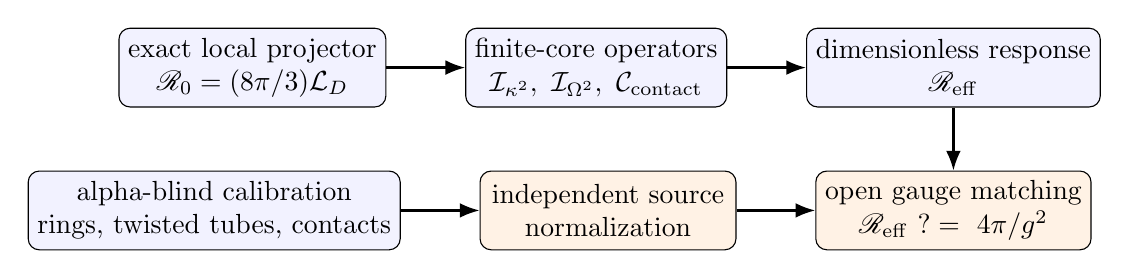
\begin{tikzpicture}[
  node distance=8mm and 10mm,
  box/.style={draw,rounded corners,align=center,minimum width=3.25cm,minimum height=1.0cm,fill=blue!5},
  open/.style={draw,rounded corners,align=center,minimum width=3.25cm,minimum height=1.0cm,fill=orange!10},
  arrow/.style={-{Latex[length=2.5mm]},thick}
]
  \node[box] (proj) {exact local projector\\$\Rgeom=(8\pi/3)\calL_D$};
  \node[box,right=of proj] (core) {finite-core operators\\$\calI_{\kappa^2},\ \calI_{\Omega^2},\ \calC_{\rm contact}$};
  \node[box,right=of core] (resp) {dimensionless response\\$\Reff$};
  \node[open,below=of resp] (gauge) {open gauge matching\\$\Reff\ ?=\ 4\pi/g^2$};
  \node[open,left=of gauge] (source) {independent source\\normalization};
  \node[box,left=of source] (data) {alpha-blind calibration\\rings, twisted tubes, contacts};
  \draw[arrow] (proj)--(core);
  \draw[arrow] (core)--(resp);
  \draw[arrow] (data)--(source);
  \draw[arrow] (source)--(gauge);
  \draw[arrow] (resp)--(gauge);
\end{tikzpicture}
\caption{Logical separation of the exact geometric term, finite-core calibration, source normalization, and the optional gauge-stiffness interpretation.  The lower-right arrow is a matching problem, not a consequence of transversality alone.}
\label{fig:logic}
\end{figure}

\section{Helicity, writhe, and material twist}
\label{sec:helicity}

The helicity of an incompressible flow is
\begin{equation}
  \calH=\int \bm u\cdot\bm\omega\,\dd^3x.
\end{equation}
For isolated thin vortex tubes, helicity is related to linking and self-linking invariants \cite{Moffatt1969,MoffattRicca1992}.  For a single framed tube of circulation $\Gamma$ in the slender-tube limit~\cite{Calugareanu1961,White1969,MoffattRicca1992},
\begin{equation}
  \frac{\calH}{\Gamma^2}=SL=Wr+Tw.
  \label{eq:calugareanu}
\end{equation}
The writhe of the centerline is the Gauss integral
\begin{equation}
  Wr[\gamma]=\frac{1}{4\pi}
  \oint\!\oint
  \frac{(\bm\gamma(s)-\bm\gamma(s'))\cdot
        [\bm t(s)\times\bm t(s')]}
       {|\bm\gamma(s)-\bm\gamma(s')|^3}
  \dd s\,\dd s'.
  \label{eq:writhe}
\end{equation}
Let $\bm d_1(s)$ be a unit material director perpendicular to $\bm t$.  Its twist rate is
\begin{equation}
  \Omega_3=(\bm t\times\bm d_1)\cdot\frac{\dd\bm d_1}{\dd s},
\end{equation}
so that
\begin{equation}
  Tw=\frac{1}{2\pi}\oint\Omega_3\,\dd s.
  \label{eq:twist}
\end{equation}
This definition remains meaningful through situations where a Frenet frame is singular or discontinuous, provided the physical material framing is specified.

\begin{figure}[t]
\centering
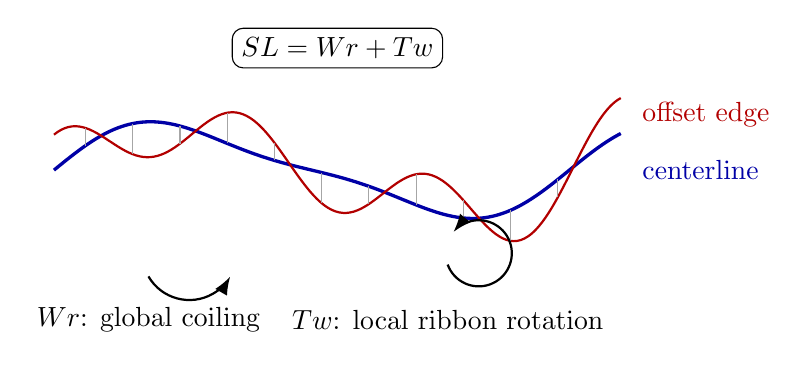
\begin{tikzpicture}[scale=1.0,>=Latex]
  \draw[very thick,blue!65!black,domain=0:7.2,samples=160,smooth,variable=\x]
    plot ({\x},{0.55*sin(55*\x)+0.15*sin(110*\x)});
  \draw[thick,red!70!black,domain=0:7.2,samples=160,smooth,variable=\x]
    plot ({\x},{0.55*sin(55*\x)+0.15*sin(110*\x)+0.45*cos(150*\x)});
  \foreach \x in {0.4,1.0,...,7.0}{
    \pgfmathsetmacro{\yc}{0.55*sin(55*\x)+0.15*sin(110*\x)}
    \pgfmathsetmacro{\yo}{0.45*cos(150*\x)}
    \draw[gray!70] (\x,\yc)--(\x,\yc+\yo);
  }
  \node[blue!65!black,anchor=west] at (7.35,0.0) {centerline};
  \node[red!70!black,anchor=west] at (7.35,0.7) {offset edge};
  \draw[->,thick] (1.2,-1.35) arc[start angle=210,end angle=330,radius=0.6];
  \node at (1.2,-1.9) {$Wr$: global coiling};
  \draw[->,thick] (5.0,-1.2) arc[start angle=200,end angle=500,radius=0.42];
  \node at (5.0,-1.9) {$Tw$: local ribbon rotation};
  \node[draw,rounded corners,fill=white] at (3.6,1.55) {$SL=Wr+Tw$};
\end{tikzpicture}
\caption{Schematic ribbon representation of self-linking.  Writhe is a nonlocal property of the centerline, while twist requires a chosen material framing.  The drawing is illustrative rather than a numerical trefoil reconstruction.}
\label{fig:ribbon}
\end{figure}

\subsection{A parity-even twist-energy bound}

Using \cref{eq:operators,eq:twist} and Cauchy--Schwarz,
\begin{align}
  (2\pi Tw)^2
  &=\left(\int_\gamma D\Omega_3\,\frac{\dd s}{D}\right)^2\nonumber\\
  &\le \left(\int_\gamma\frac{\dd s}{D}\right)
       \left(\int_\gamma(D\Omega_3)^2\frac{\dd s}{D}\right)
   =\calL_D\calI_{\Omega^2}.
\end{align}
Therefore
\begin{proposition}[Minimum material-twist energy]
For fixed $SL$, fixed centerline writhe, and fixed length,
\begin{equation}
  \boxed{
  \calI_{\Omega^2}\ge
  \frac{4\pi^2}{\calL_D}(SL-Wr)^2.}
  \label{eq:twist-bound}
\end{equation}
Equality holds if and only if $D\Omega_3$ is constant almost everywhere along the tube.
\end{proposition}

This is the appropriate way for helicity to constrain a parity-even quadratic twist term.  By contrast, $\calH/\Gamma^2$, $Wr$, and $Tw$ are pseudoscalars under spatial reflection.  A linear term
\begin{equation}
  c_H\frac{\calH}{\Gamma^2}
\end{equation}
therefore belongs to a parity-odd sector.  If such a sector admits an electromagnetic image, the natural operator class is $f_{\mu\nu}\widetilde f^{\mu\nu}$ rather than the ordinary parity-even kinetic term.  No equality between fluid helicity and a four-dimensional theta term is assumed here.

Under the additional uniform-twist approximation, \cref{eq:response-expansion} reduces to
\begin{equation}
  \Reff=\frac{8\pi}{3}\calL_D
  +c_\kappa\calI_{\kappa^2}
  +c_\Omega\frac{4\pi^2}{\calL_D}(SL-Wr)^2
  +c_C\calC_{\mathrm{contact}}+\cdots.
  \label{eq:uniform-twist-response}
\end{equation}
This is a testable ansatz, not a topological determination of $c_\Omega$.

\section{Why scalar ropelength is not a complete response observable}
\label{sec:ropelength-data}

The standard definition of ropelength is $L/\operatorname{Thi}(\gamma)$, where thickness equals the reach or normal injectivity radius for a sufficiently regular embedded curve \cite{CantarellaKusnerSullivan2002}.  Polygonal constrained-gradient methods implement the active curvature and self-distance constraints through kink and strut sets \cite{AshtonCantarellaPiatekRawdon2011}.  A scalar length can converge while the contact skeleton, multiplier measure, or local curvature structure remains unresolved.

The high-resolution trefoil computation of Przybyl and Pieranski used $200{,}640$ vertices and reported the radius-normalized estimate
\begin{equation}
  \Rop_a^{\mathrm{HR}}=32.742934477(1),
  \label{eq:HR-rop}
\end{equation}
corresponding to
\begin{equation}
  \calL_D^{\mathrm{HR}}=16.3714672385.
\end{equation}
The same study reports six finite intervals on which curvature reaches its upper bound, together with narrow torsional features and a highly structured contact set \cite{PrzybylPieranski2014}.  These are precisely the features that a core-sensitive functional may detect even when scalar ropelength has already converged.

A separate Fourier database reports~\cite{Gilbert2016}
\begin{equation}
  L=16.371637,\qquad D=1,
  \label{eq:Gilbert}
\end{equation}
which means
\begin{equation}
  \calL_D^{\mathrm{G}}=16.371637,
  \qquad
  \Rop_a^{\mathrm{G}}=32.743274.
\end{equation}
The two values are close but not identical; rounded Fourier coefficients also need not reconstruct the metadata length exactly.  They must therefore be treated as separate geometry-provenance branches rather than interchangeable inputs.

\begin{table}[t]
\caption{Trefoil geometry branches and the corresponding leading projector response.  The last two columns use the 2022 CODATA comparison value $\alpha^{-1}=137.035999177$ only after the geometric response has been fixed.}
\label{tab:trefoil-branches}
\begin{ruledtabular}
\begin{tabular}{lcccc}
Branch & $\Rop_a=L/a$ & $\calL_D=L/D$ & $(8\pi/3)\calL_D$ & $\alpha^{-1}-\Rgeom$\\
\hline
High resolution & 32.7429344770 & 16.3714672385 & 137.1532832132 & $-0.1172840362$\\
Fourier metadata & 32.7432740000 & 16.3716370000 & 137.1547054038 & $-0.1187062268$\\
\end{tabular}
\end{ruledtabular}
\end{table}

The leading high-resolution value exceeds the comparison value by approximately $855.9$ parts per million.  The Fourier-metadata branch exceeds it by approximately $866.2$ parts per million.  This proximity is a numerical coincidence unless the finite-core coefficients and the gauge normalization are independently fixed.

\section{Open gauge-stiffness matching}
\label{sec:gauge}

The transverse projector in \cref{eq:projector} is also the polarization sum for two spatially transverse modes.  This formal similarity does not establish electrodynamics.  A gauge theory additionally requires a redundancy or first-class constraint, a consistent source current, absence of a physical longitudinal photon, and agreement between static and radiative couplings.

Let $a_\mu$ be a dimensionless candidate field with
\begin{equation}
  f_{\mu\nu}=\partial_\mu a_\nu-\partial_\nu a_\mu.
\end{equation}
In a convention where the source term is normalized as $\int j^\mu a_\mu$, write
\begin{equation}
  \frac{S_{\mathrm{IR}}^{(2)}}{\hbar}
  =-\frac{\Reff}{16\pi}
   \int f_{\mu\nu}f^{\mu\nu}\,\dd^4\xi
   +\int j^\mu a_\mu\,\dd^4\xi+\cdots.
  \label{eq:IR-action}
\end{equation}
Comparison with the rescaled gauge action
\begin{equation}
  \frac{S_{\mathrm{gauge}}^{(2)}}{\hbar}
  =-\frac{1}{4g^2}\int f_{\mu\nu}f^{\mu\nu}\,\dd^4\xi
   +\int j^\mu a_\mu\,\dd^4\xi
  \label{eq:gauge-action}
\end{equation}
would imply
\begin{equation}
  \Reff=\frac{4\pi}{g^2}.
  \label{eq:stiffness}
\end{equation}
If $g^2=4\pi\alpha$ in the chosen charge convention, then $\Reff=\alpha^{-1}$.

\begin{hypothesis}[Gauge-stiffness matching]
A finite-core vortex response can be identified with an inverse electromagnetic coupling only if one microscopic model independently establishes
\begin{enumerate}[label=(\alph*)]
  \item a protected $U(1)$ gauge redundancy or equivalent first-class constraint;
  \item exactly two gapless physical transverse modes and no physical longitudinal mode;
  \item a conserved current with a fixed unit-charge normalization;
  \item the same coupling in the static interaction and radiative kinetic term;
  \item positive field energy and a causal, isotropic infrared propagation law;
  \item no use of the target coupling or an equivalent target-dependent calibration in determining $\Reff$.
\end{enumerate}
\end{hypothesis}

\subsection{Field-normalization obstruction}

The source normalization is indispensable.  Under the simultaneous rescaling
\begin{equation}
  a_\mu\mapsto\lambda a_\mu,
  \qquad
  j^\mu\mapsto\frac{1}{\lambda}j^\mu,
\end{equation}
the interaction term is unchanged, while the coefficient of $f^2$ changes.  Therefore the gauge kinetic coefficient is not an observable coupling until the normalization of the source current has been fixed independently.  A numerical coefficient close to $\alpha^{-1}$, by itself, cannot resolve this convention freedom.

The 2022 CODATA value is used here only as an external final comparison; it remains the latest CODATA adjustment available at the time of writing \cite{TiesingaEtAl2024}.  Since the low-energy electromagnetic coupling runs with scale, any proposed matching must also specify the momentum or distance regime to which it refers \cite{PeskinSchroeder1995}.

\section{Independent calibration and falsification protocol}
\label{sec:calibration}

Let the finite-core response be evaluated for a family of calibration configurations $n$.  Define
\begin{equation}
  y_n:=\Rmicro[\gamma_n,f_n,\Omega_{3,n}]
      -\frac{8\pi}{3}\calL_{D,n}
      =\sum_a A_{na}c_a+\varepsilon_n,
  \label{eq:calibration}
\end{equation}
where the columns of $A$ are the declared operator values, for example
\begin{equation}
  A_n=(\calI_{\kappa^2,n},\calI_{\Omega^2,n},\calC_{\mathrm{contact},n}).
\end{equation}
With a covariance matrix $\Sigma$, the weighted least-squares estimator is
\begin{equation}
  \widehat{\bm c}
  =(A^{\mathsf T}\Sigma^{-1}A)^{-1}
    A^{\mathsf T}\Sigma^{-1}\bm y,
  \label{eq:wls}
\end{equation}
provided the design matrix has full column rank.

The calibration set should separate the operators as directly as possible:
\begin{enumerate}[label=\textbf{C\arabic*.},leftmargin=*]
  \item \textbf{Bend response:} isolated circular finite-core rings over several $R/D$ values.  For a circle,
  \begin{equation}
    \calI_{\kappa^2}=\frac{2\pi D}{R}.
  \end{equation}
  \item \textbf{Twist response:} straight periodic tubes with several prescribed material-twist rates, with curvature and nonlocal contact absent.
  \item \textbf{Contact response:} antiparallel finite-core tube pairs over several separations, with a frozen profile and contact kernel.
  \item \textbf{Mixed holdouts:} twisted rings and curved near-contact pairs excluded from fitting.
  \item \textbf{Cross-geometry tests:} one frozen coefficient vector applied to independently reconstructed knots and links.
  \item \textbf{Final trefoil test:} only after all coefficients, conventions, and tolerances are frozen is a selected trefoil branch compared with the external target.
\end{enumerate}

Ring energy, translational speed, Kelvin-wave dispersion, and contact force may constrain the same microscopic model, but they cannot be inserted as $y_n$ unless an explicit forward derivation maps them to the same response coefficient appearing in \cref{eq:IR-action}.

\begin{figure}[t]
\centering
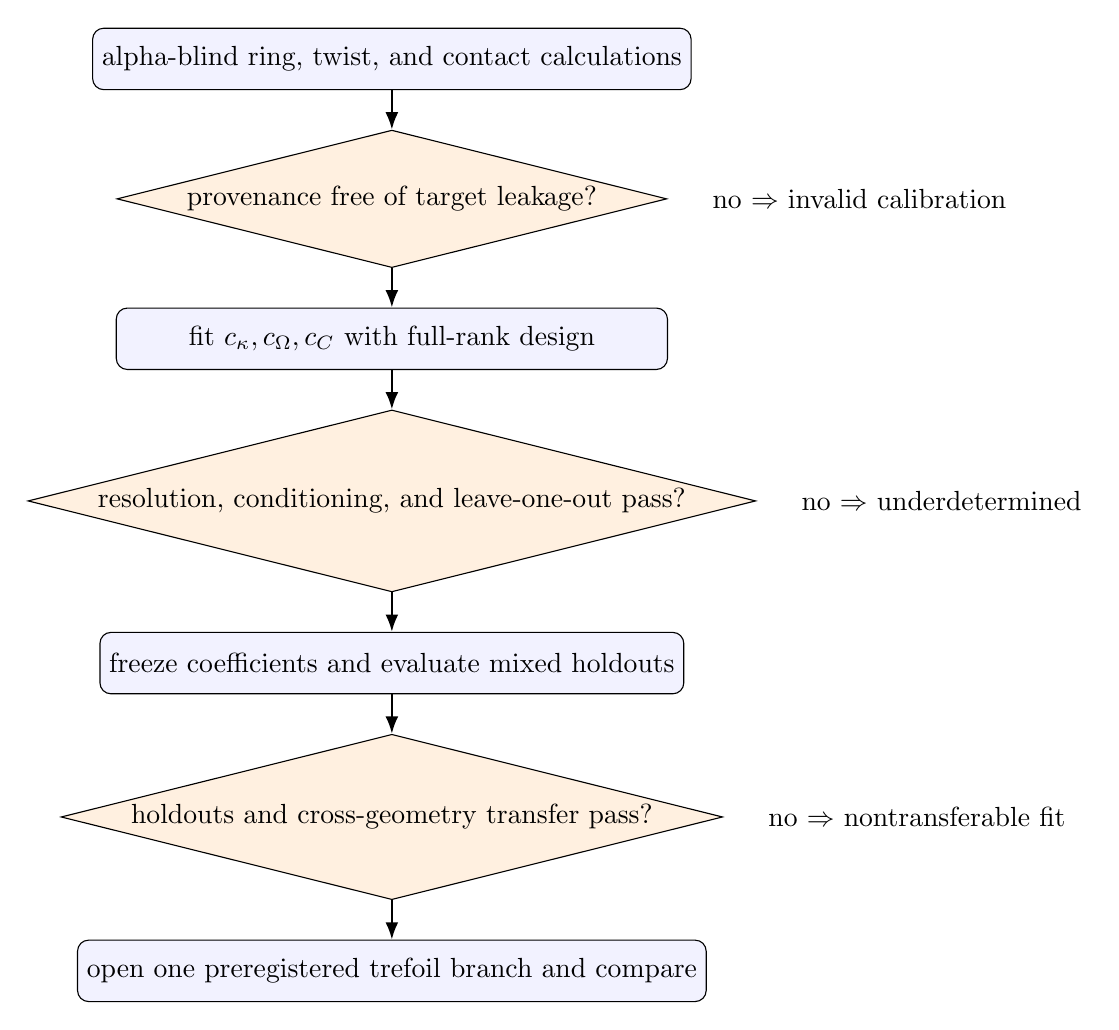
\begin{tikzpicture}[
  node distance=5mm,
  stagebox/.style={draw,rounded corners,minimum width=7.0cm,minimum height=0.78cm,align=center,fill=blue!5},
  gate/.style={draw,diamond,aspect=4,align=center,fill=orange!12,inner sep=1.5pt},
  arr/.style={-{Latex[length=2.2mm]},thick}
]
  \node[stagebox] (a) {alpha-blind ring, twist, and contact calculations};
  \node[gate,below=of a] (g0) {provenance free of target leakage?};
  \node[stagebox,below=of g0] (b) {fit $c_\kappa,c_\Omega,c_C$ with full-rank design};
  \node[gate,below=of b] (g1) {resolution, conditioning, and leave-one-out pass?};
  \node[stagebox,below=of g1] (c) {freeze coefficients and evaluate mixed holdouts};
  \node[gate,below=of c] (g2) {holdouts and cross-geometry transfer pass?};
  \node[stagebox,below=of g2] (d) {open one preregistered trefoil branch and compare};
  \draw[arr] (a)--(g0); \draw[arr] (g0)--(b);
  \draw[arr] (b)--(g1); \draw[arr] (g1)--(c);
  \draw[arr] (c)--(g2); \draw[arr] (g2)--(d);
  \node[anchor=west] at ($(g0.east)+(0.45,0)$) {no $\Rightarrow$ invalid calibration};
  \node[anchor=west] at ($(g1.east)+(0.45,0)$) {no $\Rightarrow$ underdetermined};
  \node[anchor=west] at ($(g2.east)+(0.45,0)$) {no $\Rightarrow$ nontransferable fit};
\end{tikzpicture}
\caption{Preregistered calibration and falsification sequence.  The external coupling is not consulted until the coefficients and holdout criteria have been frozen.}
\label{fig:calibration}
\end{figure}

At minimum, the following gates are required:
\begin{enumerate}[label=G\arabic*.,leftmargin=*]
  \item target exclusion throughout the transitive provenance chain;
  \item enough independent rows to leave residual degrees of freedom;
  \item full column rank and acceptable numerical conditioning;
  \item grid, core-profile, and regulator convergence;
  \item acceptable residuals and leave-one-out performance;
  \item successful mixed-geometry and cross-representation holdouts;
  \item a frozen final comparison at a preregistered tolerance.
\end{enumerate}
A successful final comparison would mean only that the declared truncation has not been falsified.  It would not establish uniqueness of the core model or prove the gauge-matching hypothesis.

\section{Discussion}
\label{sec:discussion}

The factor $8\pi/3$ has a clean and conventional origin: it is the total solid angle $4\pi$ multiplied by the isotropic mean transverse fraction $2/3$.  Its appearance in the normalized volume of a constant-radius tube is an exact algebraic equivalence.  These two derivations are mutually consistent, but both are local and both produce no curvature correction.

The physically nontrivial information begins at finite core size.  The Euler energy is nonlocal, the filament limit is singular, and regularization introduces profile-dependent data.  Tight-knot geometry adds further subtleties: minimizers are only guaranteed to be $C^{1,1}$, active contacts organize the constraint forces, and material twist cannot be reconstructed from scalar ropelength.  The high-resolution trefoil is therefore best viewed as a demanding geometry benchmark rather than as a complete dynamical state.

Helicity provides a particularly useful constraint.  It transfers global centerline writhe into material twist while preserving self-linking, but it does not set the energetic cost of that transfer.  The coefficient $c_\Omega$ remains a constitutive or microscopic response coefficient.  The bound \eqref{eq:twist-bound} is nevertheless model independent once a material framing, $SL$, $Wr$, and $\calL_D$ have been fixed.

The electromagnetic interpretation is the most restrictive step.  Transverse modes occur in many non-electromagnetic systems.  Even a Maxwell-shaped quadratic action is insufficient unless gauge redundancy, source quantization, and static--radiative universality are demonstrated.  This normalization issue is independent of the geometric coincidence and cannot be resolved by improving the trefoil ropelength alone.

\section{Conclusions}

The analysis supports five precise conclusions.
\begin{enumerate}[leftmargin=*]
  \item The isotropic incompressible projector gives the exact identity
  \begin{equation*}
    \int_{S^2}t_i(\delta_{ij}-\widehat k_i\widehat k_j)t_j\,\dd\Omega
    =\frac{8\pi}{3}.
  \end{equation*}
  \item The resulting length response is
  \begin{equation*}
    \Rgeom=\frac{8\pi}{3}\frac{L}{D}
    =\frac{4\pi}{3}\frac{L}{a}.
  \end{equation*}
  \item Neither the bare local projector nor the volume of a constant circular tube generates a curvature correction.  Nonzero corrections require finite-core or nonlocal dynamics.
  \item In a framed thin tube, helicity constrains the parity-even twist energy through
  \begin{equation*}
    \calI_{\Omega^2}\ge
    \frac{4\pi^2}{\calL_D}(SL-Wr)^2,
  \end{equation*}
  but does not determine its coefficient.
  \item Identifying a dimensionless vortex response with an inverse electromagnetic coupling remains an open matching problem that requires independent gauge and source normalization.  The nearby trefoil number is therefore a final-test target, not a derived constant.
\end{enumerate}

The immediate scientific task is not another fit to the trefoil residual.  It is the construction of an alpha-blind finite-core response calculation with enough independent geometries to determine the low-order coefficients and enough holdouts to test whether they transfer.

\begin{acknowledgments}
The author thanks the developers of the numerical ropelength and constrained-gradient literature for making high-resolution knot geometries and contact diagnostics available.  This manuscript is a reformulation of a broader exploratory programme in the language of classical fluid mechanics, geometric knot theory, and effective field theory.  All electromagnetic identifications are deliberately stated as open matching hypotheses.
\end{acknowledgments}

\appendix

\section{A schematic finite-core contact functional}

A convenient numerical contact diagnostic can be defined from a nonnegative shell kernel $K_\sigma(R)$ concentrated near the normalized diameter $R=1$ and an orthogonality weight $Q_\eta$ that selects approximately doubly critical chords:
\begin{align}
  \calC_{\mathrm{contact}}[\gamma]
  =\frac12\int\!\dd\sigma\int\!\dd\sigma'\,
  &K_\sigma\!\left(|\bm X(\sigma)-\bm X(\sigma')|\right)\nonumber\\
  &\times Q_\eta\!\left(
  \unitvec{R}\cdot\bm t(\sigma),
  \unitvec{R}\cdot\bm t(\sigma')
  \right),
  \label{eq:contact-functional}
\end{align}
where $\bm R=\bm X(\sigma)-\bm X(\sigma')$.  This is a diagnostic definition, not a universal invariant.  Its shell width, orthogonality tolerance, local-neighbor exclusion, and core profile must be frozen before calibration.  Convergence of \cref{eq:contact-functional} is a stronger requirement than convergence of scalar ropelength alone.

\section{Gauge-field rescaling}

To make the normalization obstruction explicit, start from
\begin{equation}
  S[a,j]=-\frac{1}{4g^2}\int f^2+\int j\cdot a.
\end{equation}
Set $a'=\lambda a$ and $j'=j/\lambda$.  Since $f'=\lambda f$,
\begin{equation}
  S[a',j']=-\frac{1}{4(\lambda g)^2}\int f'^2+\int j'\cdot a'.
\end{equation}
Thus the numerical value assigned to $g$ changes unless the normalization of $j$ is fixed by an independent charge convention.  This is why a geometric coefficient cannot be identified with a physical coupling from the kinetic term alone.

\begin{thebibliography}{99}

\bibitem{CantarellaKusnerSullivan2002}
J.~Cantarella, R.~B.~Kusner, and J.~M.~Sullivan,
``On the minimum ropelength of knots and links,''
\emph{Invent. Math.} \textbf{150}, 257--286 (2002),
\href{https://doi.org/10.1007/s00222-002-0234-y}{doi:10.1007/s00222-002-0234-y}.

\bibitem{AshtonCantarellaPiatekRawdon2011}
T.~Ashton, J.~Cantarella, M.~Piatek, and E.~J.~Rawdon,
``Knot tightening by constrained gradient descent,''
\emph{Exp. Math.} \textbf{20}, 57--90 (2011),
\href{https://doi.org/10.1080/10586458.2011.544581}{doi:10.1080/10586458.2011.544581}.

\bibitem{PrzybylPieranski2014}
S.~Przybyl and P.~Pieranski,
``High resolution portrait of the ideal trefoil knot,''
\emph{J. Phys. A: Math. Theor.} \textbf{47}, 285201 (2014),
\href{https://doi.org/10.1088/1751-8113/47/28/285201}{doi:10.1088/1751-8113/47/28/285201}.

\bibitem{Gilbert2016}
B.~Gilbert,
``Database of ideal knots, 3--10 crossings,'' Fourier coefficient data set
(11 June 2016), trefoil record 3:1:1.

\bibitem{Saffman1992}
P.~G.~Saffman,
\emph{Vortex Dynamics}
(Cambridge University Press, Cambridge, 1992),
\href{https://doi.org/10.1017/CBO9780511624063}{doi:10.1017/CBO9780511624063}.

\bibitem{Moffatt1969}
H.~K.~Moffatt,
``The degree of knottedness of tangled vortex lines,''
\emph{J. Fluid Mech.} \textbf{35}, 117--129 (1969),
\href{https://doi.org/10.1017/S0022112069000991}{doi:10.1017/S0022112069000991}.

\bibitem{MoffattRicca1992}
H.~K.~Moffatt and R.~L.~Ricca,
``Helicity and the C\u{a}lug\u{a}reanu invariant,''
\emph{Proc. R. Soc. Lond. A} \textbf{439}, 411--429 (1992),
\href{https://doi.org/10.1098/rspa.1992.0159}{doi:10.1098/rspa.1992.0159}.

\bibitem{Calugareanu1961}
G.~C\u{a}lug\u{a}reanu,
``Sur les classes d'isotopie des noeuds tridimensionnels et leurs invariants,''
\emph{Czech. Math. J.} \textbf{11}, 588--625 (1961).

\bibitem{White1969}
J.~H.~White,
``Self-linking and the Gauss integral in higher dimensions,''
\emph{Am. J. Math.} \textbf{91}, 693--728 (1969),
\href{https://doi.org/10.2307/2373348}{doi:10.2307/2373348}.

\bibitem{HornNicolisPenco2015}
B.~Horn, A.~Nicolis, and R.~Penco,
``Effective string theory for vortex lines in fluids and superfluids,''
\emph{J. High Energy Phys.} \textbf{2015}, 153 (2015),
\href{https://doi.org/10.1007/JHEP10(2015)153}{doi:10.1007/JHEP10(2015)153}.

\bibitem{PeskinSchroeder1995}
M.~E.~Peskin and D.~V.~Schroeder,
\emph{An Introduction to Quantum Field Theory}
(Addison--Wesley, Reading, MA, 1995).

\bibitem{TiesingaEtAl2024}
E.~Tiesinga, P.~J.~Mohr, D.~B.~Newell, and B.~N.~Taylor,
``The 2022 CODATA recommended values of the fundamental physical constants,''
NIST Standard Reference Database 121, Web Version 9.0 (2024),
\url{https://physics.nist.gov/constants}.

\end{thebibliography}

\end{document}
